\documentclass[11pt,a4paper]{article}
\usepackage{graphicx}
\usepackage{pgfgantt}

\begin{document}
\title{Courier-dependent Indirect Communication Protocol}
\author{Chen Sun}
\date{April 2014}
\maketitle

\section{Introduction}
This is MSC program final project. This project relates to Computer Security and it is mainly about designing and implementing a general use communication protocol. The rest of proposal will firstly propose the question and explain the motivation of this project by introducing and analysing some related solutions. Then a brief summary of project will convey a vague idea of this whole project. After that it will dive into the detailed plan of the project, showing the its architecture, potential challenges and methodologies. Following that a Gantt-chart of project schedule will be displayed, illustrating how the project is organized and scheduled. Finally a summary will be given to sum up the proposal.

\section{Background and Related Work}
Protocols play an extremely important role in modern communication. Different layers of protocol ensure different levels of communication safely and securely. So far, there have been hundreds of application-level protocols defined to serve various purposes of communication, from file transferring(FTP) to online chatting(XMPP). However, for most of those protocols to run, it is essential to have a stable, directly connected digital path established (like Internet, or Bluetooth) between two entities.\par
But, what if there doesn't exist such direct connection? Is there any way for those entities to communicate securely? A system called Euonym has been introduced to tackle the similar problem \cite{gregory}. It allows two relatively isolated entities to communicate through many buffering hosts connected by dynamic, unstable connections. The defect of this approach is obvious: assuming the existence of such hosts between any two random isolated entities is unrealistic and building those hosts on-the-fly will be too huge a cost.\par
A more primitive method would be using a courier to carry the message between two entities. This idea actually has been implemented thousands years ago as delivering posts and letters, and nowadays well-developed courier services cover nearly every corner of the world. However, the way of using courier services to communicate is assessed as unreliable, geographical-proximity-dependent and far way from secure \cite{horgan}. Something extra must be done if we want to achieve the communication.\par

\section{Project Summary}
Comparing to courier services mentioned above, this project proposes an enhanced solution - using a portable device as message courier to support the communication between off-line entities. Assuming there are two off-line entities Alice and Bob, and Alice wants to send Bob a message. What could happen is a portable device Courier (maybe several) copies the message from Alice, somehow transported to Bob and then deliver the message to Bob. This project aims to design and implement a protocol to allow this kind of connection established efficiently and securely.\par 
Although it will be a new protocol, the concept is very similar to Mobile Agent - a courier carries program environments from one platform to other platforms to achieve distributed computing, whose security concerns including confidentiality, integrity, accountability and availability, have been thoroughly evaluated in report Mobile Agent Security \cite{wayne}. To simplify, the basic requirements of such protocol are:
\begin{itemize}
\item The authenticity and integrity of messages are preserved during the communication
\item The confidentiality of messages between Alice and Bob are preserved even under the circumstances that the Courier could be hijacked
\item Malicious actions of Alice, Bob or Courier will be detected and rejected
\end{itemize}
\par
In this project, firstly a well-defined courier-dependent communication protocol will be designed, then programs will be developed to implement such a protocol. After that, the implementation will be tested and evaluated to show its practicality.

\section{Project Details}
\subsection{Architecture and Environment}
\begin{figure}[h!]
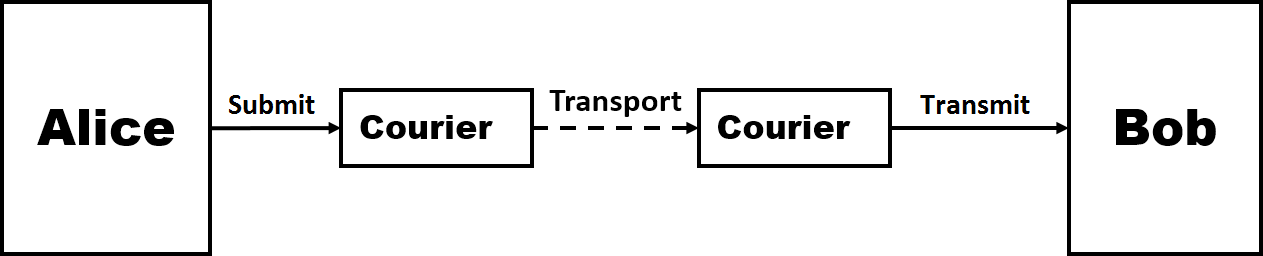
\includegraphics[width=\textwidth,natwidth=1957,natheight=256]{flowchart.png}
\caption{Simplified Scenario}
\end{figure}
As Figure 1 shows, a normal scenario will be: Alice uploads message to courier, courier transports and transmits the message to other couriers. Finally one of the couriers is transported to Bob and Bob downloads the message from that courier. Following this scenario, it separates the protocol into 3 different sub-protocols - uploading protocol, transmitting protocol and downloading protocol, and all of them will be designed consistently.\par
During the implementation phase, as off-line entities, Alice and Bob will be simulated by workstations (a laptop or desktop computer) while as portable devices, Courier will be simulated by mobile phones. So the implementation phase of this project will include programming for both computers and mobile phones. Besides, as this protocol is a very high level communication protocol, it may contain lower level protocols like TCP/IP suites or FTP as pre-work. 
\subsection{Potential Challenges}
The most challenging point of designing such protocol is that there are too many available implementations to choose, as the requirement is relatively vague. Because of this, the main difficulty lies on discussing various of different user scenarios, analysing their practicality with pros and cons, and finally producing a reasonable outcome. The fact that there is barely any pre-work of such protocol for referencing makes the mission even harder. In addition, this project also has many variants to be considered as extensions:
\begin{itemize}
\item Efficiency concerns\\
If use cryptography, it is expected to achieve relatively low overhead for encrypting/decrypting as mobile programming is involved.
\item Key revocation\\
If use cryptography, once one of the entities’ key is disclosed, it must come up with a method for new keys to be securely revoked/exchanged.
\item Deniable authentication\\
It means the participants themselves can be confident in the authenticity of origin of the messages, but they cannot prove it to a third party after the event. It also means message sender is able to deny the availability of his/her own message.
\end{itemize}

\subsection{Deliverables and Methodologies}
As mentioned before, this project mainly consists of 3 phases - protocol design, implementation and evaluation, each of them can be treated as a deliverable.

\subsubsection{Protocol Design}
In this phase a application-level communication protocol will be produced iteratively. As this protocol is designed for general use,it should both meet the basic requirements and as many user scenarios as possible. Because there may be many potential factors to be considered in real user scenario (like does Courier have to be authenticated? or which entity be the initiator?), it requires the designing phase to be responsive and iterative as new stuff will keep being added during the phase.\par
The designed protocol should be high level protocol so that it hides all implementation details behind it, such like establishing machine connections or how to encrypt and decrypt messages. It only defines the flow of actions of entities involved but nothing detail.\par
As explained, the protocol may have 3 sub-protocols so at the end of designing phase, a full set of sub-protocols will be created together with their preconditions and postconditions to support specifying their user scenario.\par

\subsubsection{Protocol Implementation}
In the implementation phase programs implement the protocol will be developed in two parts - a core protocol library for certain language and the shell. The core library defines the abstract framework of the protocol and provides essential APIs for running it. It allows different implementations of the protocol to be developed in a consistent way.\par 
Shell is the actual program that can be run on the computers or mobile phones. As the core library is just a framework, detail issues lie on the implementation of shell. There will be many choices have to be considered and balanced - like connecting method, implementation of cryptography, message format, etc.. As the program will be evaluated in the third phase, the decisions have to be wisely made to make it as efficient as possible.\par 
Similar to any software engineering processes, the implementation phase consists of program designing, implementing and testing. And at the end of this phase, a set of self-contained programs will be developed running on computers and mobile phones which simulates Alice, Bob and Couriers respectively.

\subsubsection{Software Evaluating}
Finally the programs will be ran and evaluated under different conditions to reveal the capability of this protocol. Time efficiency, memory efficiency and scalability may be the most important features of the protocol.\par 
Although the runnable program developed in this project is only one specific implementation of all possible implementations, at least such evaluation tells ``the worst" behaviour of such protocol.

\subsection{Project Schedule}
At the beginning of the project, we can roughly separate the project into following parts:
\begin{enumerate}
\item Protocol Design
\item Software Design
\item Software Development
\item Software Testing
\item Software Evalutation
\item Writting Thesis Draft
\item Thesis Modification
\end{enumerate}
Following Gantt-Chart shows the draft time schedule for the whole project:

\begin{figure}[!h]
\hspace{-1.2in}
\begin{ganttchart}[
  hgrid,
  vgrid,
  x unit=0.8cm,
  y unit title=1.2cm,
  today=1,
  today rule/.style=%
  {ultra thick}
]{1}{18}
\gantttitle{April}{1} 
\gantttitle{May}{4} 
\gantttitle{June}{4} 
\gantttitle{July}{4} 
\gantttitle{Augest}{4} 
\gantttitle{Sep}{1} \\
\gantttitlelist{4}{1}
\gantttitlelist{1,...,4}{1}
\gantttitlelist{1,...,4}{1}
\gantttitlelist{1,...,4}{1}
\gantttitlelist{1,...,4}{1}
\gantttitlelist{1}{1} \\
\ganttbar{Protocol Design}{1}{2} \\
\ganttbar{Software Design}{3}{6} \\
\ganttbar{Software Develop}{7}{11} \\
\ganttbar{Software Test}{12}{12} \\
\ganttbar{Software Evaluate}{13}{14} \\
\ganttbar{Write Draft}{15}{17} \\
\ganttbar{Modify Draft}{18}{18}
\end{ganttchart}

\caption{Project Schedule}
\end{figure}


\section{Conclusion}
To sum up, this proposal firstly raised a problem of how to achieve safe and secure communication between relatively isolated entities. Some existing solutions like building buffering hosts between or using courier service were introduced and discussed, however their serious defects stop them from being ideal. Then this project was introduced. It enhanced the traditional courier service solution by using digital couriers obeying specific communication protocol. Designing such protocol was the major aim of this project. Besides the aim and objective of the project, this proposal also revealed some detail by showing the basic architecture of the protocol, analysing potential challenges and explaining different project phases and deliverables. At last, the proposal split the project into number of reasonable steps and gave a rough time schedule for undertaking this project. 


\begin{thebibliography}{9}
\bibitem{gregory}
  Gregory Kempe, Norman C. Hutchinson.
  \emph{Networks without Borders: Communication despite Disconnection}.
  \emph{PROC}. AICT/ICIW, 0-7695-2522-9/06.
  2006.


\bibitem{horgan}
  Horgan et al. (2010).
  \emph{METHOD AND APPARATUS FOR SECURE COMMUNICATIONS}.
  US Patent: 7,743,247 B1.

\bibitem{wayne}
  Wayne Jansen, Tom Karygiannis.
  \emph{Mobile Agent Security}.
  NIST Special Publication 800-19.
  1999.
  

\end{thebibliography}
\end{document}